%\documentclass{beamer}
%\usetheme{Pittsburgh}
\documentclass{scrartcl}

\usepackage[utf8]{inputenc}
\usepackage{default}
\usepackage[procnames]{listings}
\usepackage{graphicx}
%\usepackage[toc,page]{appendix}
\usepackage{caption}
\usepackage{hyperref}
\usepackage{color}
%\usepackage{csvsimple}
\usepackage{float}
%\usepackage[T1]{fontenc}



%Bibliogrpahy?
%\usepackage{bibentry}
%\nobibliography*
%\bibentry{ }


%Python
\definecolor{keywords}{RGB}{255,0,90}
\definecolor{comments}{RGB}{0,0,113}
\definecolor{red}{RGB}{160,0,0}
\definecolor{green}{RGB}{0,150,0}
\lstset{language=Python,
    basicstyle=\ttfamily\scriptsize,
    keywordstyle=\color{keywords},
    commentstyle=\color{comments},
    stringstyle=\color{red},
    identifierstyle=\color{green},
    breaklines = true,
    columns=fullflexible,
    %Numbering and tabs
    %numbers=left,
    %numberstyle=\tiny\color{gray},
    %stepnumber=2,
    %numbersep=1em,
    tabsize=4,
    showspaces=false,
    showstringspaces=false}

\begin{document}

\title{Learning and Adaptivity}
\subtitle{Report No. 3}
\author{
  \href{daiem.ali@smail.inf.h-brs.de}{Ali, Daiem}: \href{https://github.com/daiemna}{github.com/daiemna}\\
  \href{christophe.quignon@smail.inf.h-brs.de}{Quignon, Christophe}:\href{https://github.com/ChrisQuignon}{github.com/ChrisQuignon}
  %Familyname, Name
}
\date{\today}


\maketitle

%TODO: add abstract and conclusion
%labels (or zero)
%references (or zero)
%remove scaffolding code


\begin{abstract}
%TODO :review this!
\textbf{Abstract:} This week we trained Random Forest for regression analysis of time series data. The data was preprocessed and then given to the regression algorithm, then root mean squared error(RMSE) for each predicted series is computed. The affect of time over prediction's RMSE was analysed to determine "when do we need to retrain our model?"
\end{abstract}


\section{Project introduction}
%Include an introduction section to your project
Heat pumps are a sustainable way to transfer thermal energy into out away from builds to keep a comfortable temperature. But to operate a heating pump is not a trivial task, different building distribute the heat differently and weather with its chaotic nature has a major influence on the temperature flow. In addition, they suffer from a suboptimal efficiency because they often have a bad time delay from sensing to acting. This could be counteracted by predicting future temperatures to overact sensors. efficiency could be increased by predicting energy consumption and delay that to times where energy is cheap. 
Thus we want to predict the behaviour or an energy pump with respect to the weather.


\section{Time Series Data Preprocessing}
%
The time series data was forward-filled and to replace missing readings with previous readings, this caused the hourly energy readings to be constant for 1 hour. Then it was re-sampled over 5 minutes time interval by taking mean of the interval data and if any data entry had a 'NaN' or 'Inf' the whole row was dropped. \par

The time interval for training and testing was selected, the training data was first six months data form 1st of July 2014 at 00:00 to 1st of December 2014 at 00:00 and the reaming two months data(from 1st of December 2014 at 00:01 to 1st of February 2015 at 00:01) was to be used as testing data. To assess the deterioration of fitted model with respect to time the testing data was varied and explained in next section.

\section{Prediction Analysis}
%
First the fitted model was asked to predict next 1 hour data and then next 2 hour data and so on up till next 100 hours data. which resulted in following plot \ref{fig:hourly_time_delta}:

\begin{figure}[H]
  \centering
  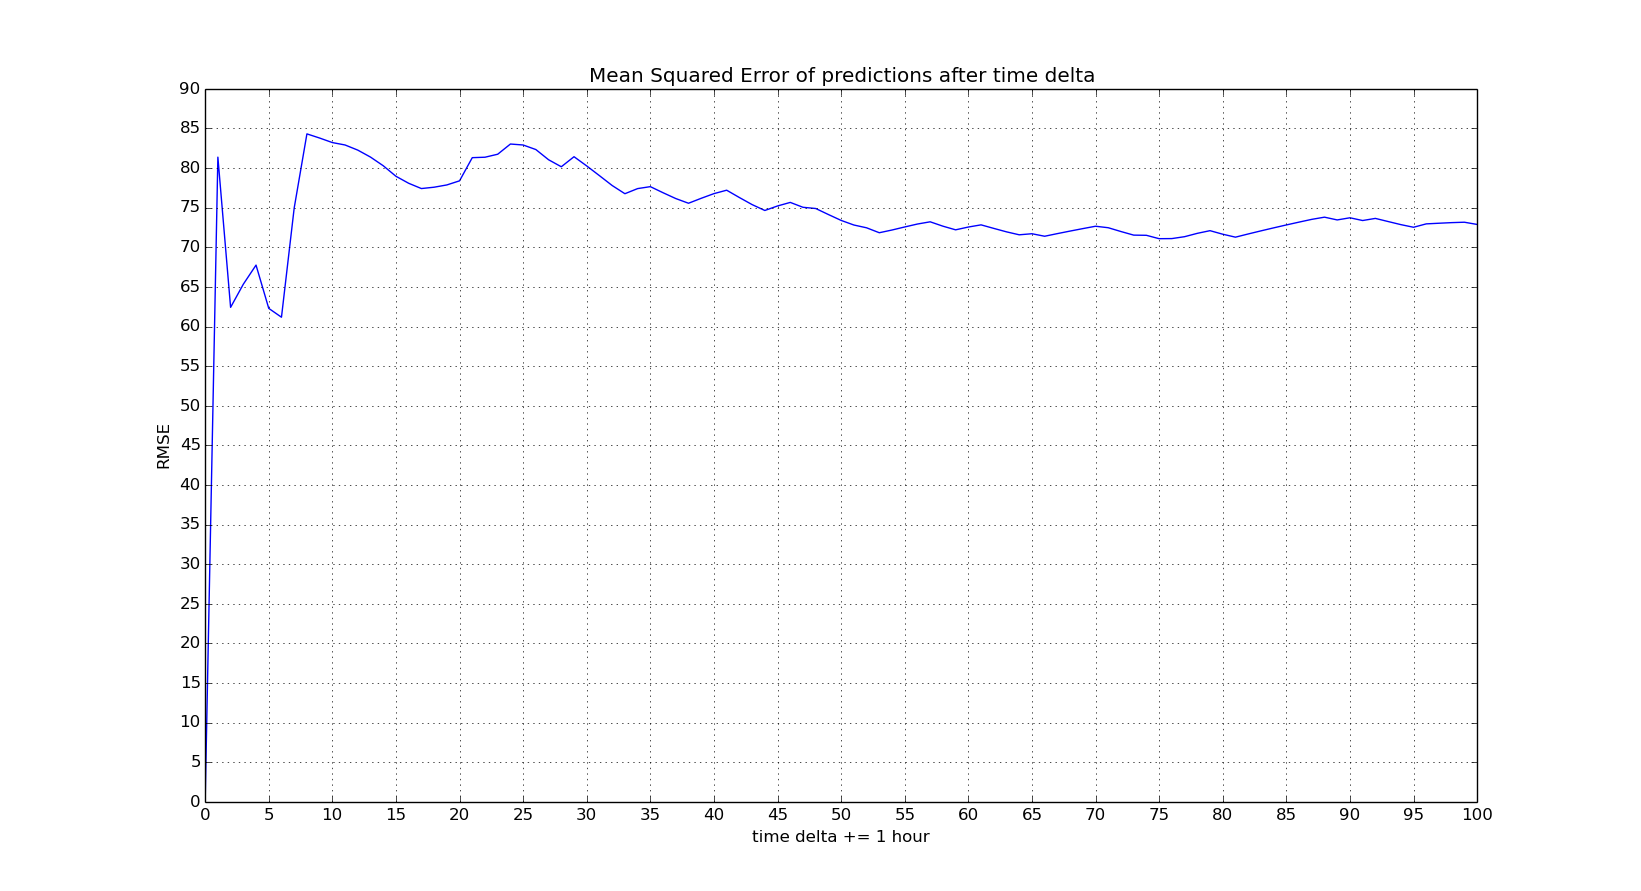
\includegraphics[width=1\linewidth]{img/hourly_time_delta_test.png}
  \caption[This is needed]{RMSE of time series prediction where time ranges varies for t+1h,t+2h ... t+100h where h=hours.\footnotemark}
  \label{fig:hourly_time_delta}
\end{figure}
\newpage
Secondly, the model predicted the next 1 day data and then 2 days data and so on up till 60 days(2 months) data, which is depicted in the following figure \ref{fig:daily_time_delta}

\begin{figure}[H]
  \centering
  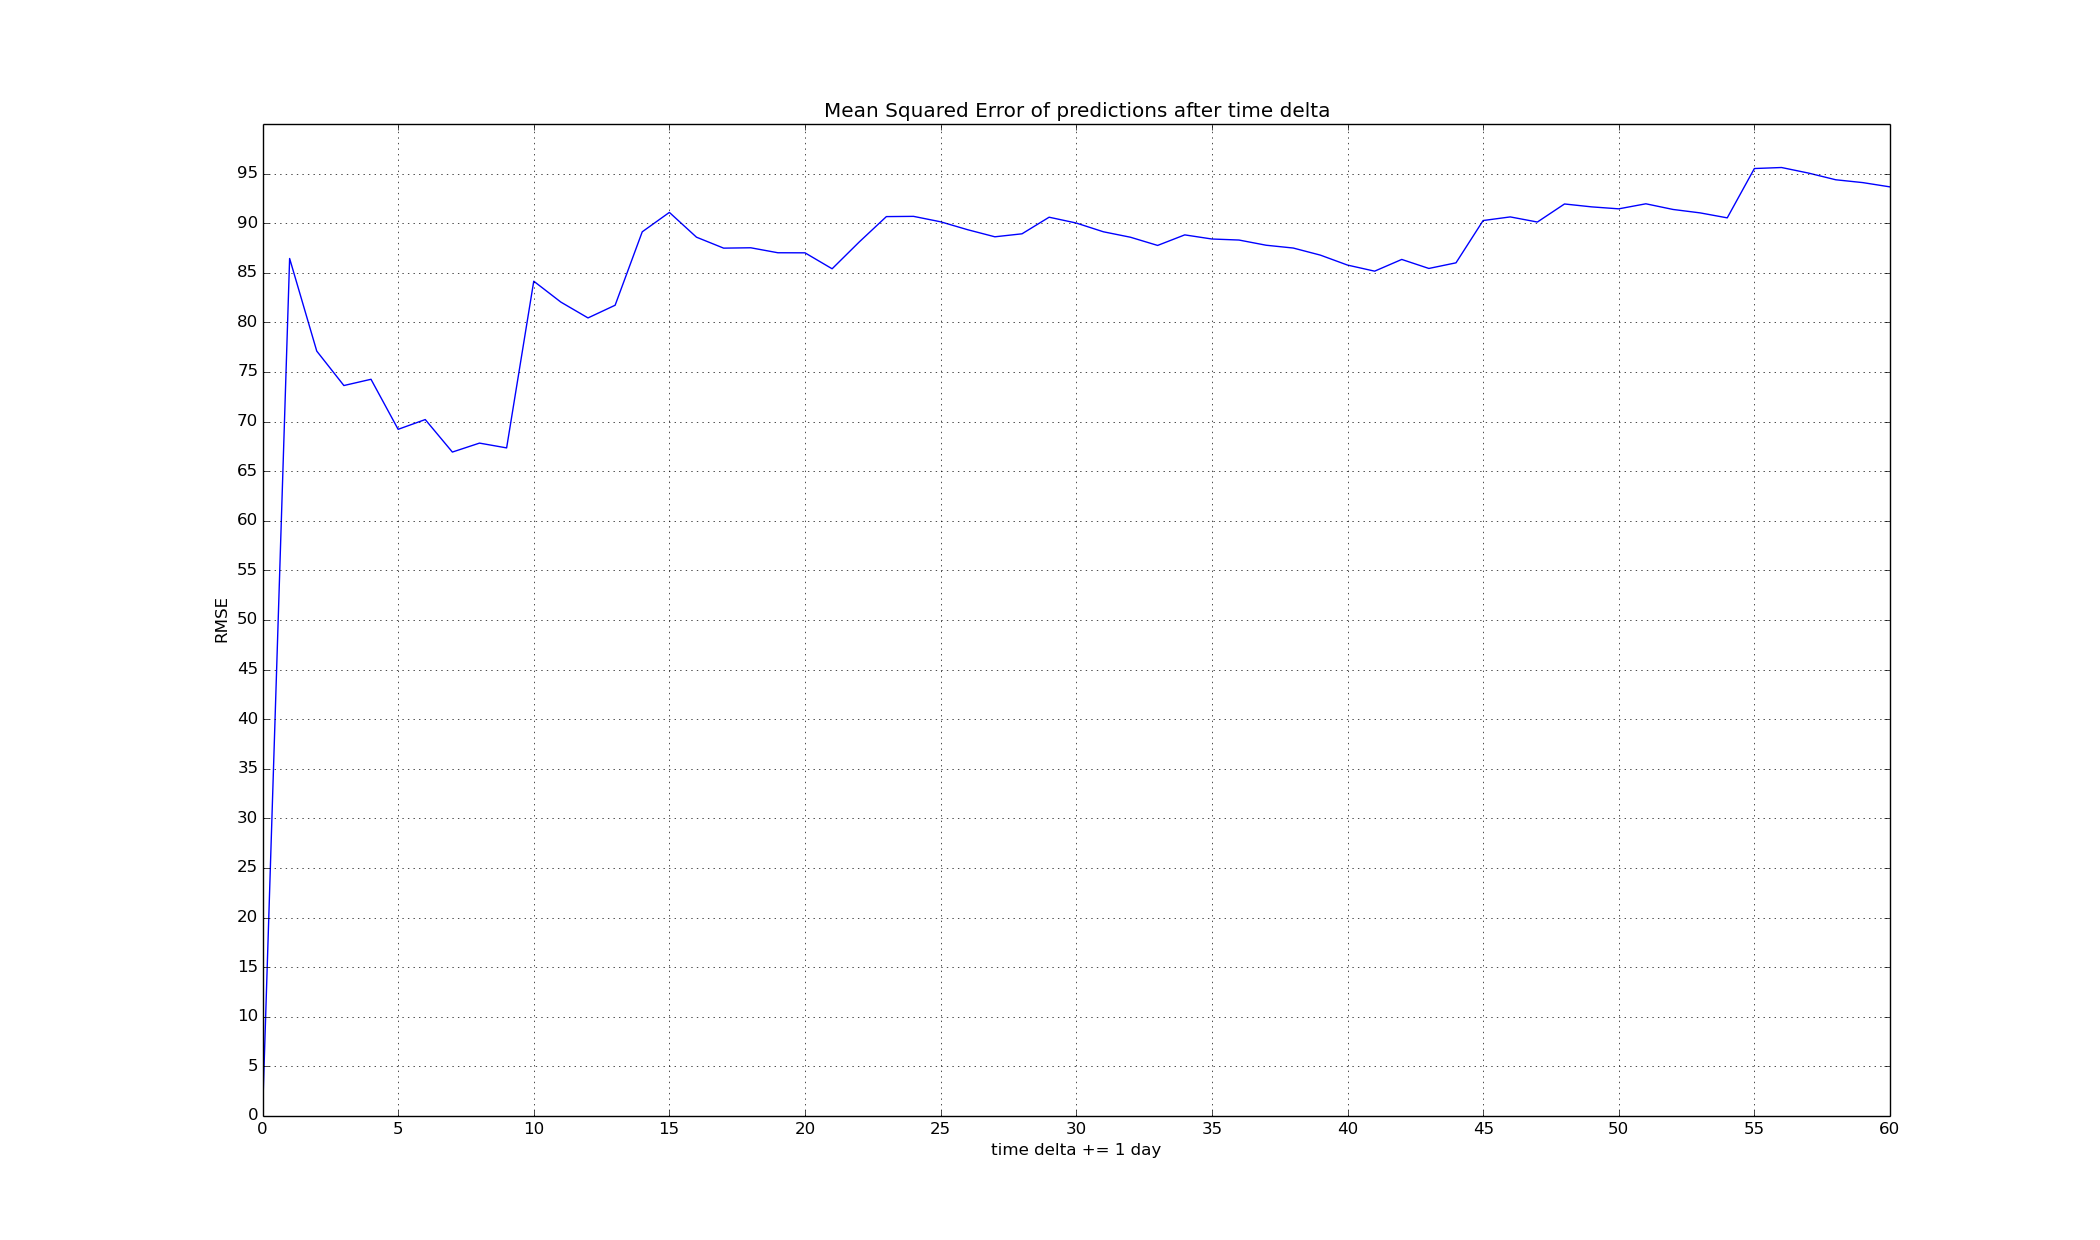
\includegraphics[width=1\linewidth]{img/daily_time_delta_test.png}
  \caption[This is needed]{RMSE of time series prediction where time ranges varies for t+1d,t+2d ... t+60d where d=days.\footnotemark}
  \label{fig:daily_time_delta}
\end{figure}
\section{Conclusion} 
%TODO
%http://blog.kaggle.com/2012/05/01/chucking-everything-into-a-random-forest-ben-hamner-on-winning-the-air-quality-prediction-hackathon/
The hourly analysis shows that the model gets really worst after 6 hours of prediction and then starts improving till later 100 hours(approx. 4 days). From the \ref{fig:daily_time_delta} we can observe that the prediction deteriorate 

%BIBLIOGRPAHY?
\bibliographystyle{plain}%amsalpha
\bibliography{bib.bib}
%\bibentry{}

%\begin{appendix}
%\section{}

%\end{appendix}


%COPY AND PASTE FROM HERE

%\begin{enumerate}
% \item
%\end{enumerate}

%\href{link}{text}

%\begin[Language=Python]{lstlisting}
%#PYTHON CODE HERE
%\end{lstlisting}

%\lstinputlisting[language=Python]{	}

%\csvautotabular[separator=semicolon]{data.csv}

%\subsubsection{left}
%\begin{figure}[H]
%  \centering
%  \includegraphics[width=0.5\linewidth]{../img/	}
%  %\caption{}
%  %\label{fig:}
%\end{figure}
%PUT UNITS ON THE FIGURES

\end{document}
